\documentclass[12pt,a4paper]{article}

% Packages
\usepackage[utf8]{inputenc}
\usepackage[margin=1in]{geometry}
\usepackage{amsmath}
\usepackage{amssymb}
\usepackage{graphicx}
\usepackage{hyperref}
\usepackage{listings}
\usepackage{xcolor}
\usepackage{tikz}
\usepackage{pgfplots}
\usepackage{algorithm}
\usepackage{algpseudocode}
\usepackage{booktabs}
\usepackage{caption}
\usepackage{subcaption}

\pgfplotsset{compat=1.18}
\usetikzlibrary{positioning,shapes.geometric,arrows.meta,calc,decorations.pathreplacing}

% Hyperref setup
\hypersetup{
    colorlinks=true,
    linkcolor=blue,
    filecolor=magenta,      
    urlcolor=cyan,
    pdftitle={Neural Networks from Scratch},
    pdfpagemode=FullScreen,
}

% Code listing style
\lstset{
    language=Python,
    basicstyle=\ttfamily\footnotesize,
    keywordstyle=\color{blue},
    commentstyle=\color{gray},
    stringstyle=\color{red},
    numbers=left,
    numberstyle=\tiny\color{gray},
    stepnumber=1,
    numbersep=5pt,
    backgroundcolor=\color{white},
    showspaces=false,
    showstringspaces=false,
    showtabs=false,
    frame=single,
    tabsize=2,
    captionpos=b,
    breaklines=true,
    breakatwhitespace=false,
    escapeinside={\%*}{*)},
    xleftmargin=2em,
    framexleftmargin=1.5em
}

\title{\textbf{Neural Networks from Scratch}\\
\Large A Comprehensive Deep Learning Framework Made From Scratch in Python}
\author{\url{https://github.com/Mondonno/} (Mikolaj Mocek)}
\date{\today}

\begin{document}

\maketitle

% GitHub Repository Link - Large and Visible
\begin{center}
\fcolorbox{blue}{blue!10}{
    \parbox{0.9\textwidth}{
        \centering
        \Huge\textbf{\href{https://github.com/Mondonno/nns}{%
            \textcolor{blue}{GitHub Repository}}}\\[0.3cm]
        \large\texttt{https://github.com/Mondonno/nns}
    }
}
\end{center}

\vspace{0.5cm}

\begin{abstract}
This document presents a comprehensive implementation of neural networks built entirely from scratch in Python. The project provides a modular, extensible framework for understanding the mathematical foundations and algorithmic details of deep learning, including automatic differentiation through backpropagation, various optimization algorithms, and rigorous gradient verification. This implementation prioritizes educational clarity and mathematical rigor over computational efficiency, making it ideal for research, education, and gaining deep insights into neural network internals.
\end{abstract}

\tableofcontents
\newpage

%==============================================================================
\section{Introduction}

Neural networks have revolutionized machine learning and artificial intelligence, yet their inner workings often remain obscured by high-level frameworks. This project implements neural networks from first principles without relying on external deep learning libraries such as TensorFlow or PyTorch. By building every component from the ground up—from basic activation functions to complex layers—this framework reveals the mathematical elegance and computational challenges underlying modern deep learning systems.

\subsection{Project Motivation}

While production deep learning frameworks offer optimized implementations, they abstract away crucial details that are essential for:
\begin{itemize}
    \item \textbf{Deep Understanding}: Grasping the mathematical foundations of backpropagation
    \item \textbf{Research Innovation}: Experimenting with novel architectures and algorithms
    \item \textbf{Educational Value}: Teaching and learning neural network fundamentals
    \item \textbf{Debugging Skills}: Understanding where and why things can go wrong
\end{itemize}

\subsection{Key Design Principles}

\begin{enumerate}
    \item \textbf{Modularity}: Each component (layers, functions, optimizers) is independently testable
    \item \textbf{Transparency}: Mathematical operations are explicit and well-documented
    \item \textbf{Extensibility}: Easy to add custom layers, activation functions, and optimizers
    \item \textbf{Verification}: Built-in gradient checking ensures correctness
\end{enumerate}

%==============================================================================
\section{Project Architecture}

The framework is organized into a hierarchical module structure that mirrors the conceptual organization of neural networks.

\subsection{High-Level Structure}

\begin{figure}[h]
\centering
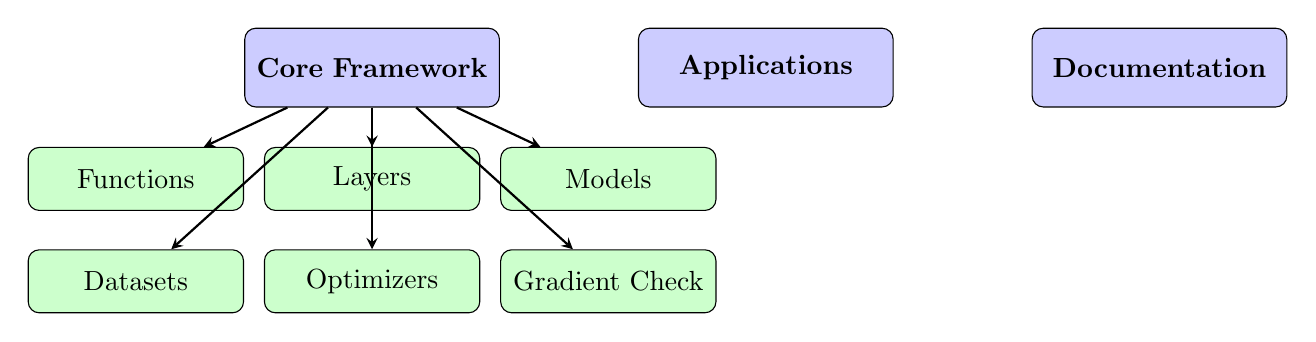
\begin{tikzpicture}[
    module/.style={rectangle, draw, fill=blue!20, text width=3cm, text centered, rounded corners, minimum height=1cm},
    submodule/.style={rectangle, draw, fill=green!20, text width=2.5cm, text centered, rounded corners, minimum height=0.8cm},
    arrow/.style={->,>=stealth,thick}
]

% Main modules
\node[module] (core) at (0,0) {\textbf{Core Framework}};
\node[module] (nns) at (5,0) {\textbf{Applications}};
\node[module] (docs) at (10,0) {\textbf{Documentation}};

% Core submodules
\node[submodule, below=0.5cm of core, xshift=-3cm] (functions) {Functions};
\node[submodule, below=0.5cm of core, xshift=0cm] (layers) {Layers};
\node[submodule, below=0.5cm of core, xshift=3cm] (models) {Models};
\node[submodule, below=1.8cm of core, xshift=-3cm] (datasets) {Datasets};
\node[submodule, below=1.8cm of core, xshift=0cm] (optimizers) {Optimizers};
\node[submodule, below=1.8cm of core, xshift=3cm] (gradient) {Gradient Check};

% Arrows
\draw[arrow] (core) -- (functions);
\draw[arrow] (core) -- (layers);
\draw[arrow] (core) -- (models);
\draw[arrow] (core) -- (datasets);
\draw[arrow] (core) -- (optimizers);
\draw[arrow] (core) -- (gradient);

\end{tikzpicture}
\caption{High-level architecture of the neural network framework}
\end{figure}

\subsection{Module Description}

\subsubsection{Functions Module}
Implements mathematical operations including:
\begin{itemize}
    \item \textbf{Activation Functions}: ReLU, Sine, Linear, Sine-squared
    \item \textbf{Loss Functions}: Mean Squared Error (MSE)
    \item \textbf{Operations}: 2D Convolution
\end{itemize}

\subsubsection{Layers Module}
Neural network building blocks:
\begin{itemize}
    \item \textbf{Dense}: Fully connected layers with configurable neurons
\end{itemize}

\subsubsection{Models Module}
High-level model abstractions:
\begin{itemize}
    \item \textbf{Sequential}: Linear stack of layers
    \item \textbf{Optimizers}: Momentum, NAG, Gradient Clipping
\end{itemize}

\subsubsection{Datasets Module}
Data handling and preprocessing:
\begin{itemize}
    \item \textbf{Dataset}: Base class with batching and shuffling
    \item \textbf{Transforms}: Min-max scaling and other preprocessing
\end{itemize}

%==============================================================================
\section{Mathematical Foundations}

\subsection{Forward Propagation}

For a neural network with $L$ layers, the forward pass computes:

\begin{align}
\mathbf{z}^{[l]} &= \mathbf{W}^{[l]} \mathbf{a}^{[l-1]} + \mathbf{b}^{[l]} \\
\mathbf{a}^{[l]} &= g^{[l]}(\mathbf{z}^{[l]})
\end{align}

where:
\begin{itemize}
    \item $\mathbf{z}^{[l]}$ is the pre-activation (weighted sum) at layer $l$
    \item $\mathbf{a}^{[l]}$ is the activation output at layer $l$
    \item $\mathbf{W}^{[l]}$ and $\mathbf{b}^{[l]}$ are weights and biases
    \item $g^{[l]}$ is the activation function
\end{itemize}

\subsection{Backpropagation}

The gradient of the loss $\mathcal{L}$ with respect to the weights is computed via the chain rule:

\begin{align}
\frac{\partial \mathcal{L}}{\partial \mathbf{W}^{[l]}} &= \frac{\partial \mathcal{L}}{\partial \mathbf{z}^{[l]}} \frac{\partial \mathbf{z}^{[l]}}{\partial \mathbf{W}^{[l]}} = \delta^{[l]} (\mathbf{a}^{[l-1]})^T \\
\frac{\partial \mathcal{L}}{\partial \mathbf{b}^{[l]}} &= \delta^{[l]} \\
\delta^{[l]} &= \frac{\partial \mathcal{L}}{\partial \mathbf{z}^{[l]}} = (\mathbf{W}^{[l+1]})^T \delta^{[l+1]} \odot g'^{[l]}(\mathbf{z}^{[l]})
\end{align}

where $\delta^{[l]}$ is the error term at layer $l$ and $\odot$ denotes element-wise multiplication.

\subsection{Gradient Descent Update}

Weights are updated using the computed gradients:

\begin{equation}
\mathbf{W}^{[l]} \leftarrow \mathbf{W}^{[l]} - \alpha \frac{\partial \mathcal{L}}{\partial \mathbf{W}^{[l]}}
\end{equation}

where $\alpha$ is the learning rate.

%==============================================================================
\section{Core Components Implementation}

\subsection{Function Base Class}

All mathematical operations inherit from a base \texttt{Function} class:

\begin{lstlisting}[caption={Function base class defining the interface for all operations}]
class Function():
    def __init__(self):
        self.name = self.__class__.__name__
    
    def call(self, input):
        raise Exception("Must implement call method")
    
    def derivative(self, input):
        raise Exception("Must implement derivative method")
\end{lstlisting}

This design ensures every function implements both forward computation and its derivative for backpropagation.

\subsection{Dense Layer Implementation}

The fully connected layer is the fundamental building block:

\begin{lstlisting}[caption={Key methods of the Dense layer (simplified)}]
class Dense(Layer):
    def __init__(self, inputsCount, neuronsCount, activation):
        self.neuronsCount = neuronsCount
        self.inputsCount = inputsCount
        self.weights = [[init_weight() 
            for j in range(inputsCount + 1)] 
            for i in range(neuronsCount)]
        self.activation = activation
    
    def forwardPass(self, inputs):
        # Compute weighted sum: z = Wx + b
        weightedSum = self.weightedSum(inputs)
        # Apply activation: a = g(z)
        outputs = [self.activation.call(z) 
                   for z in weightedSum]
        return inputs, outputs
    
    def backwardPass(self, inputs, errorDerivatives):
        # Compute gradients via chain rule
        # Returns: (weight_gradients, next_layer_errors)
        ...
\end{lstlisting}

\subsection{Sequential Model}

The Sequential model orchestrates the training loop:

\begin{lstlisting}[caption={Sequential model training (core structure)}]
class Sequential(Model):
    def fit(self, dataset, epochs=1):
        for epoch in range(epochs):
            for batch in dataset.generate():
                for inputs, targets in batch:
                    # Forward pass
                    outputs = self.forwardPass(inputs)
                    
                    # Compute error
                    error = self.error.call((outputs, targets))
                    
                    # Backward pass
                    for layer in reversed(self.layers):
                        gradients = layer.backwardPass(...)
                        
                    # Update weights
                    self.updateWeights(gradients)
\end{lstlisting}

%==============================================================================
\section{Gradient Verification}

A critical feature of this framework is built-in gradient checking to verify the correctness of analytical gradients computed through backpropagation.

\subsection{Numerical Gradient Approximation}

The centered difference formula provides accurate numerical gradients:

\begin{equation}
\frac{\partial f}{\partial x} \approx \frac{f(x + \varepsilon) - f(x - \varepsilon)}{2\varepsilon}
\end{equation}

This method has error $O(\varepsilon^2)$, significantly better than one-sided differences with $O(\varepsilon)$ error.

\subsection{Relative Error Metric}

To compare analytical and numerical gradients:

\begin{equation}
\text{relative error} = \frac{|\nabla_a - \nabla_n|}{\max(|\nabla_a|, |\nabla_n|, \varepsilon)}
\end{equation}

\begin{table}[h]
\centering
\caption{Gradient verification error thresholds}
\begin{tabular}{@{}ll@{}}
\toprule
\textbf{Relative Error} & \textbf{Assessment} \\ \midrule
$< 10^{-7}$ & Excellent \checkmark \\
$< 10^{-5}$ & Good \checkmark \\
$< 10^{-3}$ & Acceptable \\
$> 10^{-3}$ & Likely bug $\times$ \\ \bottomrule
\end{tabular}
\end{table}

\subsection{Gradient Checking Workflow}

\begin{figure}[h]
\centering
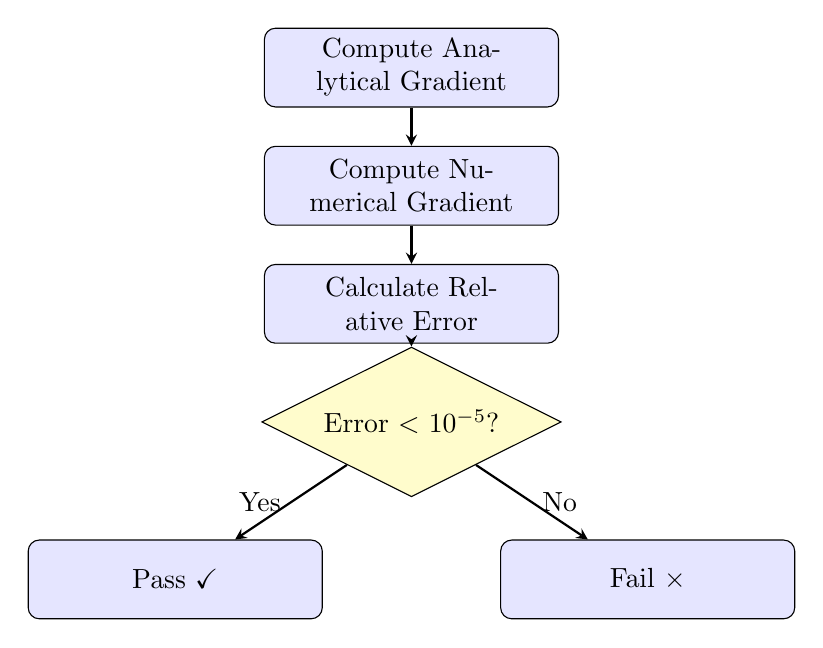
\begin{tikzpicture}[node distance=1.5cm,
    box/.style={rectangle, draw, fill=blue!10, text width=3.5cm, text centered, rounded corners, minimum height=1cm},
    decision/.style={diamond, draw, fill=yellow!20, text width=2.5cm, text centered, aspect=2},
    arrow/.style={->,>=stealth,thick}
]

\node[box] (compute) {Compute Analytical Gradient};
\node[box, below of=compute] (numerical) {Compute Numerical Gradient};
\node[box, below of=numerical] (compare) {Calculate Relative Error};
\node[decision, below of=compare] (check) {Error $< 10^{-5}$?};
\node[box, below of=check, yshift=-0.5cm, xshift=-3cm] (pass) {Pass \checkmark};
\node[box, below of=check, yshift=-0.5cm, xshift=3cm] (fail) {Fail $\times$};

\draw[arrow] (compute) -- (numerical);
\draw[arrow] (numerical) -- (compare);
\draw[arrow] (compare) -- (check);
\draw[arrow] (check) -- node[left] {Yes} (pass);
\draw[arrow] (check) -- node[right] {No} (fail);

\end{tikzpicture}
\caption{Gradient verification workflow}
\end{figure}

%==============================================================================
\section{Build Process and Setup}

\subsection{System Requirements}

\begin{itemize}
    \item \textbf{Python}: 3.8 or higher
    \item \textbf{Dependencies}: matplotlib (for visualization)
    \item \textbf{Operating System}: Platform-independent (Linux, macOS, Windows)
\end{itemize}

\subsection{Installation Steps}

\begin{enumerate}
    \item \textbf{Clone the repository}:
    \begin{lstlisting}[language=bash, numbers=none]
git clone https://github.com/Mondonno/nns.git
cd nns
    \end{lstlisting}

    \item \textbf{Install dependencies}:
    \begin{lstlisting}[language=bash, numbers=none]
pip install -r requirements.txt
    \end{lstlisting}

    \item \textbf{Verify installation with tests}:
    \begin{lstlisting}[language=bash, numbers=none]
pytest
    \end{lstlisting}
\end{enumerate}

\subsection{Testing Framework}

The project uses pytest for comprehensive testing:

\begin{lstlisting}[language=bash, numbers=none, caption={Running tests}]
# Run all tests
pytest

# Run gradient checking tests
pytest core/test_gradient_check.py -v

# Run layer tests
pytest core/layers/ -v

# Run with coverage
pytest --cov=core
\end{lstlisting}

\subsection{Basic Usage Example}

\begin{lstlisting}[caption={Training a simple neural network}]
from core.models.sequential import Sequential
from core.layers.dense import Dense
from core.functions.relu import RectifiedLinearFunction
from core.functions.mse import MSEFunction
from core.functions.linear import LinearFunction

# Define network architecture
model = Sequential([
    Dense(2, 4, RectifiedLinearFunction()),
    Dense(4, 1, LinearFunction())
], MSEFunction(), learning_rate_function)

# Train on dataset
model.fit(dataset, epochs=1000)

# Make predictions
predictions = model.forwardPassByOutputLayer(test_inputs)
\end{lstlisting}

%==============================================================================
\section{Project Evolution}

\subsection{Development Timeline}

The project evolved through several major phases, each adding significant functionality:

\begin{figure}[h]
\centering
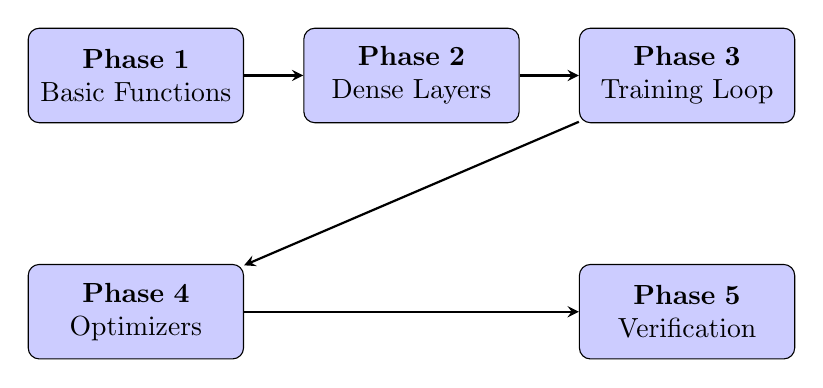
\begin{tikzpicture}[
    phase/.style={rectangle, draw, fill=blue!20, text width=2.5cm, text centered, rounded corners, minimum height=1.2cm},
    arrow/.style={->,>=stealth,thick}
]

\node[phase] (p1) at (0,0) {\textbf{Phase 1}\\Basic Functions};
\node[phase] (p2) at (3.5,0) {\textbf{Phase 2}\\Dense Layers};
\node[phase] (p3) at (7,0) {\textbf{Phase 3}\\Training Loop};
\node[phase] (p4) at (0,-3) {\textbf{Phase 4}\\Optimizers};
\node[phase] (p5) at (7,-3) {\textbf{Phase 5}\\Verification};

\draw[arrow] (p1) -- (p2);
\draw[arrow] (p2) -- (p3);
\draw[arrow] (p3) -- (p4);
\draw[arrow] (p4) -- (p5);

\end{tikzpicture}
\caption{Project development phases}
\end{figure}

\subsubsection{Phase 1: Foundation (Basic Functions)}

The project began with implementing fundamental mathematical operations:
\begin{itemize}
    \item Base \texttt{Function} class architecture
    \item Activation functions (Linear, ReLU, Sine)
    \item Loss functions (MSE)
    \item Forward and derivative computation
\end{itemize}

\textbf{Key Challenge}: Designing a flexible interface that would support all future operations.

\subsubsection{Phase 2: Neural Network Layers}

Building upon functions, the layer abstraction emerged:
\begin{itemize}
    \item \texttt{Layer} base class
    \item Dense (fully connected) layer implementation
    \item Weight initialization strategies
    \item Forward pass through multiple neurons
\end{itemize}

\textbf{Key Challenge}: Handling arbitrary input/output dimensions efficiently.

\subsubsection{Phase 3: Training Infrastructure}

With layers functional, the training loop was implemented:
\begin{itemize}
    \item Sequential model for layer stacking
    \item Backpropagation algorithm implementation
    \item Gradient computation through chain rule
    \item Weight update mechanism
\end{itemize}

\textbf{Key Challenge}: Correctly implementing the backpropagation algorithm and ensuring gradient flow through all layers.

\subsubsection{Phase 4: Optimization Algorithms}

Enhanced training with advanced optimizers:
\begin{itemize}
    \item Momentum optimizer for accelerated convergence
    \item Nesterov Accelerated Gradient (NAG)
    \item Gradient clipping for stability
    \item Learning rate scheduling
\end{itemize}

\textbf{Key Challenge}: Maintaining optimizer state across training iterations.

\subsubsection{Phase 5: Verification and Testing}

Critical quality assurance phase:
\begin{itemize}
    \item Numerical gradient checking implementation
    \item Comprehensive test suite with pytest
    \item Gradient verification for all components
    \item Documentation and examples
\end{itemize}

\textbf{Key Challenge}: Ensuring numerical stability and gradient correctness across all operations.

\subsection{Architecture Evolution}

\begin{table}[h]
\centering
\caption{Component count evolution}
\begin{tabular}{@{}lcccc@{}}
\toprule
\textbf{Component} & \textbf{Phase 2} & \textbf{Phase 4} & \textbf{Phase 5} \\ \midrule
Functions & 3 & 5 & 7 \\
Layers & 1 & 2 & 5 \\
Optimizers & 0 & 3 & 3 \\
Tests & 0 & 2 & 8 \\
Lines of Code & ~200 & ~800 & ~2500 \\ \bottomrule
\end{tabular}
\end{table}

%==============================================================================
\section{Key Features and Innovations}

\subsection{Modular Design}

Every component implements a clean interface:
\begin{itemize}
    \item \textbf{Functions}: \texttt{call()} and \texttt{derivative()} methods
    \item \textbf{Layers}: \texttt{forwardPass()} and \texttt{backwardPass()} methods
    \item \textbf{Models}: \texttt{fit()} for training, \texttt{forwardPassByOutputLayer()} for inference
\end{itemize}

\subsection{Extensibility}

Adding new components requires minimal code:

\begin{lstlisting}[caption={Adding a custom activation function}]
from core.functions.function import Function

class TanhFunction(Function):
    def call(self, x):
        return (exp(x) - exp(-x)) / (exp(x) + exp(-x))
    
    def derivative(self, x):
        tanh_x = self.call(x)
        return 1 - tanh_x ** 2
\end{lstlisting}

\subsection{Gradient Verification System}

The built-in gradient checker validates implementations:
\begin{itemize}
    \item Compares analytical vs numerical gradients
    \item Tests at multiple input points
    \item Provides detailed error reports
    \item Catches implementation bugs early
\end{itemize}

\subsection{Initialization Strategies}

Support for multiple weight initialization methods:
\begin{itemize}
    \item \textbf{Xavier Initialization}: $W \sim \mathcal{N}(0, \sqrt{2/(n_{in} + n_{out})})$
    \item \textbf{Random Initialization}: Uniform distribution
    \item \textbf{Custom Initializers}: User-defined initialization functions
\end{itemize}

%==============================================================================
\section{Network Architectures}

\subsection{Fully Connected Network}

\begin{figure}[h]
\centering
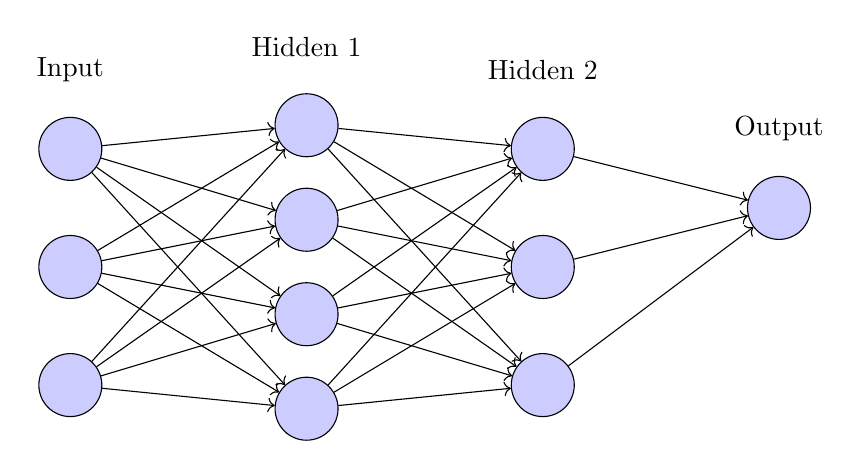
\begin{tikzpicture}[
    neuron/.style={circle, draw, minimum size=0.8cm, fill=blue!20},
    layer/.style={rectangle, draw=none},
]

% Input layer
\foreach \i in {1,2,3}
    \node[neuron] (I\i) at (0,-\i*1.5) {};
\node[layer, above of=I1] {Input};

% Hidden layer 1
\foreach \i in {1,2,3,4}
    \node[neuron] (H1\i) at (3,-\i*1.2) {};
\node[layer, above of=H11] {Hidden 1};

% Hidden layer 2
\foreach \i in {1,2,3}
    \node[neuron] (H2\i) at (6,-\i*1.5) {};
\node[layer, above of=H21] {Hidden 2};

% Output layer
\node[neuron] (O1) at (9,-2.25) {};
\node[layer, above of=O1] {Output};

% Connections
\foreach \i in {1,2,3}
    \foreach \j in {1,2,3,4}
        \draw[->] (I\i) -- (H1\j);

\foreach \i in {1,2,3,4}
    \foreach \j in {1,2,3}
        \draw[->] (H1\i) -- (H2\j);

\foreach \i in {1,2,3}
    \draw[->] (H2\i) -- (O1);

\end{tikzpicture}
\caption{Fully connected neural network architecture (3-4-3-1)}
\end{figure}

%==============================================================================
\section{Performance Considerations}

\subsection{Computational Complexity}

For a dense layer with $n_{in}$ inputs and $n_{out}$ outputs:

\begin{itemize}
    \item \textbf{Forward Pass}: $O(n_{in} \times n_{out})$ operations
    \item \textbf{Backward Pass}: $O(n_{in} \times n_{out})$ operations
    \item \textbf{Memory}: $O(n_{in} \times n_{out})$ for weights
\end{itemize}

\subsection{Optimization Opportunities}

While this implementation prioritizes clarity, several optimizations are possible:

\begin{enumerate}
    \item \textbf{Vectorization}: Replace loops with NumPy array operations
    \item \textbf{GPU Acceleration}: Port computations to CUDA
    \item \textbf{Memory Pooling}: Reuse memory across operations
    \item \textbf{Mixed Precision}: Use FP16 for faster training
    \item \textbf{Quantization}: Reduce model size with INT8 weights
\end{enumerate}

%==============================================================================
\section{Practical Applications}

\subsection{Example: XOR Problem}

The classic XOR problem demonstrates the necessity of hidden layers:

\begin{lstlisting}[caption={Training a network to learn XOR}]
# XOR dataset
dataset = Dataset([
    ([0, 0], [0]),
    ([0, 1], [1]),
    ([1, 0], [1]),
    ([1, 1], [0])
], batch_size=4)

# Network architecture
model = Sequential([
    Dense(2, 4, RectifiedLinearFunction()),
    Dense(4, 1, LinearFunction())
], MSEFunction(), learning_rate)

# Train
model.fit(dataset, epochs=1000)
\end{lstlisting}

%==============================================================================
\section{Lessons Learned}

\subsection{Technical Insights}

\begin{enumerate}
    \item \textbf{Numerical Stability}: Careful handling of floating-point arithmetic is crucial
    \item \textbf{Gradient Verification}: Essential for catching subtle bugs in backpropagation
    \item \textbf{Weight Initialization}: Poor initialization can prevent learning entirely
    \item \textbf{Learning Rate}: Single most important hyperparameter to tune
\end{enumerate}

\subsection{Software Engineering}

\begin{enumerate}
    \item \textbf{Abstraction}: Clean interfaces enable easy testing and extension
    \item \textbf{Testing}: Comprehensive tests catch regressions early
    \item \textbf{Documentation}: Good documentation accelerates development
    \item \textbf{Incremental Development}: Build and test small components first
\end{enumerate}

%==============================================================================
\section{Future Directions}

Potential extensions to the framework:

\begin{itemize}
    \item \textbf{Convolutional Neural Networks}: 2D convolution operations and layers (currently in development)
    \item \textbf{Recurrent Neural Networks}: LSTM and GRU layers
    \item \textbf{Attention Mechanisms}: Self-attention and transformer blocks
    \item \textbf{Batch Normalization}: Improve training stability
    \item \textbf{Dropout}: Regularization for better generalization
    \item \textbf{Advanced Optimizers}: Adam, RMSprop, AdaGrad
    \item \textbf{Data Augmentation}: Expand dataset with transformations
    \item \textbf{Visualization Tools}: Plot loss curves and activations
    \item \textbf{Model Serialization}: Save and load trained models
\end{itemize}

%==============================================================================
\section{Conclusion}

This project demonstrates that building neural networks from scratch is not only feasible but highly educational. By implementing every component—from basic activation functions to complex convolutional layers—we gain deep insights into the mathematical foundations and computational challenges of deep learning.

The modular architecture ensures that the framework is extensible and maintainable, while the comprehensive test suite and gradient verification provide confidence in the correctness of the implementation. Although not optimized for production use, this framework serves its primary purpose: enabling deep understanding of neural network internals.

The evolution of the project, from simple functions to complete neural networks, mirrors the historical development of deep learning itself, making it an ideal educational tool for anyone seeking to understand how modern AI systems work at a fundamental level.


%==============================================================================
\appendix

\section{Code Repository Structure}

Complete directory tree of the project:

\begin{verbatim}
nns/
|---- LICENSE
|---- README.md
|---- requirements.txt
|---- pytest.ini
|---- main.tex                    # This document
|---- core/                       # Core framework
|   |---- __init__.py
|   |---- dict.py
|   |---- gradient_check.py       # Gradient verification
|   |---- test_gradient_check.py
|   |---- functions/              # Activation and loss functions
|   |   |---- __init__.py
|   |   |---- function.py         # Base class
|   |   |---- linear.py
|   |   |---- relu.py
|   |   |---- sine.py
|   |   |---- mse.py
|   |   `---- convolute.py
|   |---- layers/                 # Neural network layers
|   |   |---- __init__.py
|   |   |---- layer.py            # Base class
|   |   |---- dense.py            # Fully connected
|   |   |---- convolution2d.py    # Convolutional
|   |   |---- maxpool2d.py        # Max pooling
|   |   |---- flatten.py          # Reshaping
|   |   |---- test_dense.py
|   |   |---- test_convolution2d.py
|   |   `---- initializators/     # Weight initialization
|   |       |---- function.py
|   |       `---- xavier.py
|   |---- models/                 # Model architectures
|   |   |---- __init__.py
|   |   |---- model.py            # Base class
|   |   |---- sequential.py       # Sequential model
|   |   `---- optimizers/         # Optimization algorithms
|   |       |---- __init__.py
|   |       |---- function.py
|   |       |---- momentum.py
|   |       |---- nag.py
|   |       `---- clipping.py
|   `---- datasets/               # Data handling
|       |---- __init__.py
|       |---- dataset.py
|       |---- file_dataset.py
|       |---- image_dataset.py
|       `---- transforms/
|           `---- min_max.py
|---- nns/                        # Applications
|   |---- main.py
|   |---- conv2d.py
|   `---- playground.py
|---- perceptron/                 # Simple examples
|   `---- main.py
`---- docs/                       # Documentation
    |---- ivus/
    |---- medium/
    `---- quarkml/
\end{verbatim}

\section{Testing Guide}

\subsection{Running Tests}

Execute the test suite with various options:

\begin{lstlisting}[language=bash, numbers=none]
# Run all tests with verbose output
pytest -v

# Run specific test file
pytest core/test_gradient_check.py

# Run tests with coverage report
pytest --cov=core --cov-report=html

# Run tests matching a pattern
pytest -k "gradient"
\end{lstlisting}

\subsection{Test Categories}

The test suite includes:
\begin{itemize}
    \item \textbf{Unit Tests}: Individual function and layer tests
    \item \textbf{Integration Tests}: Full model training tests
    \item \textbf{Gradient Tests}: Numerical verification of all components
    \item \textbf{Edge Cases}: Boundary conditions and error handling
\end{itemize}

%==============================================================================

\vspace{1cm}
\begin{center}
\rule{0.9\textwidth}{0.4pt}\\[0.3cm]
\textbf{Repository:} \href{https://github.com/Mondonno/nns}{\texttt{github.com/Mondonno/nns}}
\end{center}

\end{document}
